\documentclass[10pt,oneside]{article}

\usepackage[T1]{fontenc}
\usepackage{fontawesome}

\usepackage[paper=a4paper,margin=2cm,bottom=2.5cm]{geometry}
\usepackage[sfdefault,light,condensed]{roboto}
\usepackage[export]{adjustbox}
\usepackage[usenames,dvipsnames,table]{xcolor}

\usepackage{amsmath,amssymb,array,fancyhdr,graphicx,enumitem,lastpage,multicol,tabularx,textcomp,titlesec}
\usepackage{mathtools}

\setlength\extrarowheight{1pt}
\setlength\parindent{0cm}
\renewcommand\headrule{}
\setlength{\footskip}{1.25cm}

\pagestyle{fancy}

\definecolor{BoxHeaderBG}{RGB}{50, 50, 50}
\definecolor{BoxHeaderText}{RGB}{255, 255, 255}

\newcommand{\BoxHeader}[2]{
    \multicolumn{#1}{| >{\bfseries\footnotesize\cellcolor{BoxHeaderBG}\arraybackslash}l |}{
        \textcolor{BoxHeaderText}{#2}
    }
}

\definecolor{ATLHeaderBG}{RGB}{65, 190, 30}
\definecolor{ATLHeaderText}{RGB}{0, 0, 0}

\definecolor{ATLSkillBG}{RGB}{215, 230, 210}
\definecolor{ATLSkillText}{RGB}{0, 0, 0}

\definecolor{DefinitionBoxHeaderBG}{RGB}{30, 30, 110}
\definecolor{DefinitionBoxHeaderText}{RGB}{255, 255, 255}

\definecolor{FormativeHeaderBG}{RGB}{150, 30, 150}
\definecolor{FormativeHeaderText}{RGB}{255, 255, 255}

\definecolor{GlobalContextHeaderBG}{RGB}{255, 255, 150}
\definecolor{GlobalContextHeaderText}{RGB}{0, 0, 0}

\definecolor{KeyConceptHeaderBG}{RGB}{15, 225, 225}
\definecolor{KeyConceptHeaderText}{RGB}{0, 0, 0}

\definecolor{RelatedConceptHeaderBG}{RGB}{15, 170, 170}
\definecolor{RelatedConceptHeaderText}{RGB}{0, 0, 0}

\definecolor{QuestionHeaderBG}{RGB}{240, 240, 240}
\definecolor{QuestionHeaderText}{RGB}{0, 0, 0}

\definecolor{SolutionHeaderBG}{RGB}{225, 150, 110}
\definecolor{SolutionHeaderText}{RGB}{0, 0 , 0}

\definecolor{SummativeHeaderBG}{RGB}{195, 15, 15}
\definecolor{SummativeHeaderText}{RGB}{255, 255, 255}

\newcommand{\ATLHeader}[1]{
    \cellcolor{ATLHeaderBG}\textcolor{ATLHeaderText}{
        \bfseries\footnotesize
        ATL SKILL (#1) \hfill \faGears
    }
}

\newcommand{\ATLSkill}[1]{
    \cellcolor{ATLSkillBG}\textcolor{ATLSkillText}{
        \itshape #1
    }
}

\newcommand{\DefinitionBoxHeader}{
    \cellcolor{DefinitionBoxHeaderBG}\textcolor{DefinitionBoxHeaderText}{
        \bfseries\footnotesize
        DEFINITIONS \hfill \faPencil
    }
}

\newcommand{\FormativeHeader}{
    \cellcolor{FormativeHeaderBG}\textcolor{FormativeHeaderText}{
        \bfseries\footnotesize
        FORMATIVE ASSESSMENT \hfill \faComments
    }
}

\newcommand{\GlobalContextHeader}[1]{
    \cellcolor{GlobalContextHeaderBG}\textcolor{GlobalContextHeaderText}{
        \bfseries\footnotesize
        GLOBAL CONTEXT (#1) \hfill \faGlobe
    }
}

\newcommand{\KeyConceptHeader}[1]{
    \cellcolor{KeyConceptHeaderBG}\textcolor{KeyConceptHeaderText}{
        \bfseries\footnotesize
        KEY CONCEPT (#1) \hfill \faKey
    }
}

\newcommand{\RelatedConceptHeader}[1]{
    \cellcolor{RelatedConceptHeaderBG}\textcolor{RelatedConceptHeaderText}{
        \bfseries\footnotesize
        RELATED CONCEPT (#1) \hfill \faLink
    }
}

\newcommand{\SolutionHeader}[1]{
    \cellcolor{SolutionHeaderBG}\textcolor{SolutionHeaderText}{
        \bfseries\footnotesize 
        #1 \hfill \faPaste
    }
}

\newcommand{\SummativeHeader}{
    \cellcolor{SummativeHeaderBG}\textcolor{SummativeHeaderText}{
        \bfseries\footnotesize
        SUMMATIVE ASSESSMENT \hfill \faCheck
    }
}

\newcounter{QuestionCounter}

\newcommand{\QuestionBox}[1]{
    \stepcounter{QuestionCounter}
    \cellcolor{QuestionHeaderBG}\textcolor{QuestionHeaderText}{
        {\bfseries\scriptsize Q\theQuestionCounter} #1
    }
}

\newcommand{\boxwidth}{\linewidth}

\lhead{\scriptsize\texttt{U\UnitNumber: \UnitTitle \\ L\LessonNumber: \LessonTitle}}
\rhead{\scriptsize\ttfamily [DESIGN/\CourseName/U\UnitNumber/L\LessonNumber]\\\ }

\lfoot{
\includegraphics[height=2cm,valign=c]{Files/logo}}
\cfoot{\footnotesize DESIGN/\CourseName/U\UnitNumber/L\LessonNumber\ | \LessonTitle \\ Woodstock School | Mussoorie, Uttarakhand, India}
\rfoot{
\includegraphics[height=2cm,valign=c]{Files/ib-world-school-logo-1-colour}}

\titleformat{\section}{\normalfont\Large\bfseries}{}{0em}{}[{\titlerule[0.5pt]}]
\titleformat{\subsection}{\normalfont\large\bfseries}{}{0em}{}


\usepackage{circuitikz}
\usetikzlibrary{arrows}

\def\CourseName{MYP3}

\def\LessonNumber{04}
\def\LessonTitle{Variable Resistance}

\def\UnitNumber{01}
\def\UnitTitle{Circuits \& Electronics}

\begin{document}
    % Core Components (Remove when no longer required!)
    \thispagestyle{empty}
    \begin{tabularx}{\boxwidth}{| X | }
        \hline
        \ATLHeader{} \\\hline
        \ATLSkill{} \\\hline
        \QuestionBox{} \\\hline
    \end{tabularx}

    \begin{tabularx}{\boxwidth}{| X |}
        \hline
        \DefinitionBoxHeader \\\hline
    \end{tabularx}

    \begin{tabularx}{\boxwidth}{| X |}
        \hline
        \GlobalContextHeader{}\\\hline
    \end{tabularx}

    \begin{tabularx}{\boxwidth}{| X |}
        \hline
        \KeyConceptHeader{} \\\hline
    \end{tabularx}

    \begin{tabularx}{\boxwidth}{| X |}
        \hline
        \RelatedConceptHeader{} \\\hline
    \end{tabularx}

    \begin{tabularx}{\boxwidth}{| X |}
        \hline
        \SolutionHeader{SOLUTION} \\\hline
    \end{tabularx}

    \begin{tabularx}{\boxwidth}{| X | }
        \hline
        \FormativeHeader \\\hline
        \QuestionBox{} \\\hline
    \end{tabularx}

    \begin{tabularx}{\boxwidth}{| X |}
        \hline
        \SummativeHeader \\\hline
        \QuestionBox{}\\\hline
    \end{tabularx}

    \newpage

    \begin{center}
        \huge\bfseries
        \LessonTitle
    \end{center}

    \section{Before You Begin}

    \pagebreak

    \section{Technical Background}

    \subsection{Variable Resistors}
    \subsubsection*{Potentiometer}

    \subsubsection*{Photoresistor}

    \pagebreak

    \section{Developing Technical Skills}
    \subsection{Circuit \#11}
    Our first circuit this lesson will use the photoresistor to provide variable resistance for the circuit.

    \subsubsection*{You Will Need}
    \begin{itemize}[noitemsep]
        \item[(1)] CR2032 Battery
        \item[(1)] Photoresistor/LDR
        \item[(1)] LED
        \item[(1)] Roll of Copper Tape
        \item[(1)] Roll of Cellophane Tape   
    \end{itemize}

    \subsubsection*{Directions}
    Create the following paper circuit, then wave your hand over the LDR to observe the effects of variable resistance on the LED.

    \bigskip\medskip
    \begin{center}
        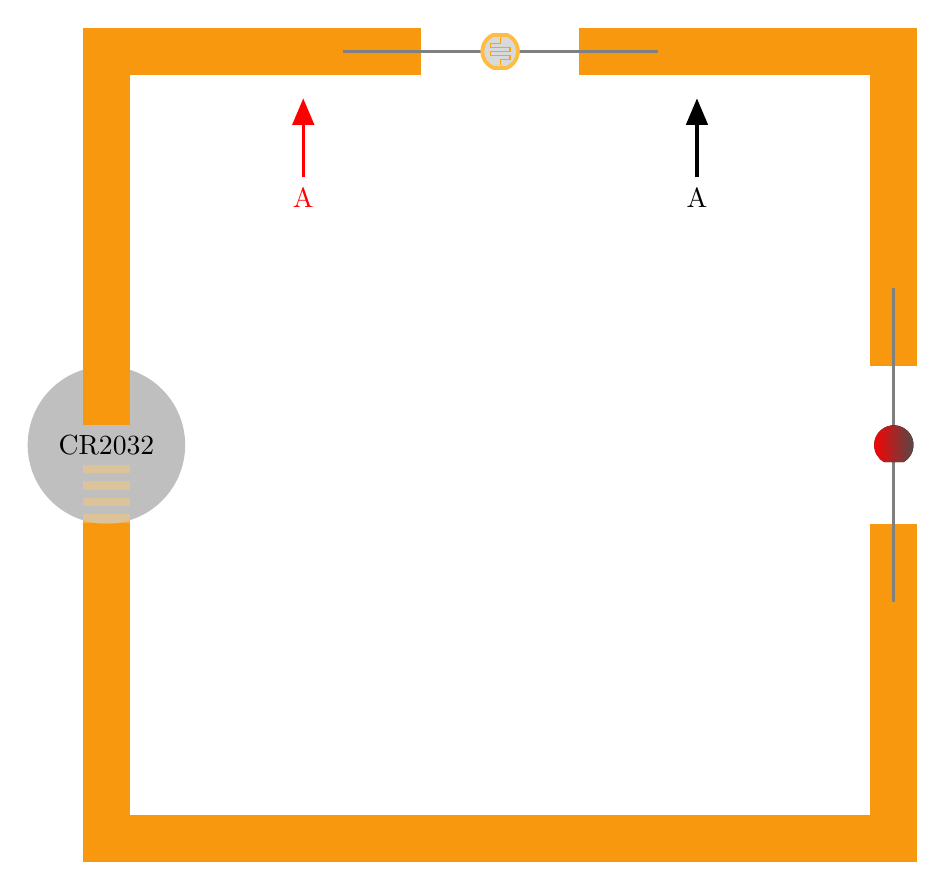
\begin{tikzpicture}
            \draw[line width=6mm,YellowOrange] (0, 1) |- (4, 5)
                                                (6, 5) -| (10, 1)
                                                (10,-1) |- (0, -5) -- (0, 0);
                                                ;

            \begin{scope}[xshift=5cm,yshift=5cm]   % Photoresistor / LDR
                \draw[black!50,very thick] (-2, 0) -- (2, 0);
                \clip (-0.25, -0.23) rectangle (0.25, 0.23);
                \fill[fill=Orange!75] (0, 0) circle (0.25);
                \clip (-0.2, -0.175) rectangle (0.2, 0.175);
                \fill[fill=black!15] (0, 0) circle (0.2);
                \draw[Orange] (0, 0.175) -- (0, 0.1) -- (-0.125, 0.1) -- (-0.125, 0.05) -- (0.125, 0.05) -- (0.125, 0) -- (-0.125, 0) -- (-0.125, -0.05) -- (0.125, -0.05) -- (0.125, -0.1) -- (0, -0.1) -- (0, -0.175);
            \end{scope}

            \fill[black!25] (0, 0) circle (10mm);            
            \draw[line width=6mm, dashed,YellowOrange!50,draw opacity=0.5] (0, -0.25) -- (0, -1);
            \draw[line width=6mm,YellowOrange] (0, 0.25) -- (0, 1);
            \node[align=center] at (0, 0) {CR2032};

            \draw[very thick,black!50] (10, 2) -- (10, -2);
            \fill[left color=red, right color=black!70] ([shift=(-60:2.5mm)]10,0) arc (-60:240:2.5mm);


            \draw[->,>=triangle 45,very thick,red] (2.5, 3.4) node[below] {A} -- (2.5, 4.4);
            \draw[->,>=triangle 45,very thick,black] (7.5, 3.4) node[below] {A} -- (7.5, 4.4);
        \end{tikzpicture}
    \end{center}

    \bigskip
    \begin{tabularx}{\boxwidth}{| X |}
        \hline
        \ATLHeader{Communication Skills}\\\hline
        \ATLSkill{...make inferences and draw conclusions...}\\\hline
        \QuestionBox{Use a multimeter to measure the resistance of the LDR in the above circuit as the light entering it changes. Do the results agree with your idea of how this variable resistor works? Why or why not?}\\\hline
        \ \\[3cm]\hline
    \end{tabularx}
    
    \pagebreak
    \subsection{Circuit \#12}
    The following circuit will allow you to explore the behaviours of the potentiometer, particularly as you turn it in each direction.

    \subsubsection*{You Will Need}
    \begin{itemize}[noitemsep]
        \item[(1)] CR2032 Battery
        \item[(1)] Potentiometer
        \item[(2)] LEDs
        \item[(1)] Roll of Copper Tape
        \item[(1)] Roll of Cellophane Tape    
    \end{itemize}

    \subsubsection*{Directions}
    Create the following paper circuit and manipulate the potentiometer to observe its effects on the two LEDs.

    \medskip
    \textbf{Note:} The gaps between the terminals of the potentiometer are necessary. You may need to trim your copper tape slightly if you are having trouble leaving enough space.

    \bigskip
    \begin{center}
        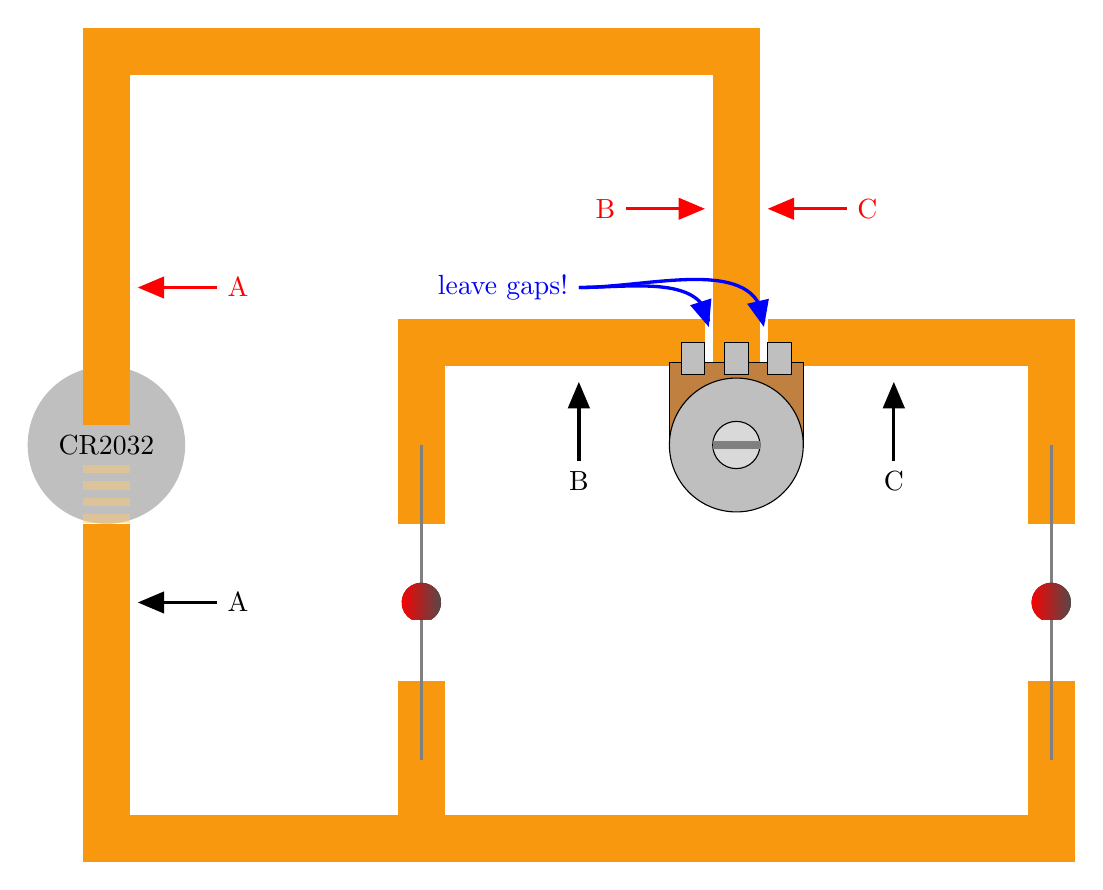
\begin{tikzpicture}
            \draw[line width=6mm,YellowOrange] (0, 1) |- (8, 5) -- (8, 0);
            \draw[line width=6mm,YellowOrange] (0, -1) |- (12, -5) -- (12, -3);
            \draw[line width=6mm,YellowOrange] (4, -5) -- (4, -3);
            \draw[line width=6mm,YellowOrange] (7.6, 1.3) -| (4, -1);
            \draw[line width=6mm,YellowOrange] (8.4, 1.3) -| (12, -1);

            \fill[black!25] (0, 0) circle (10mm);            
            \draw[line width=6mm, dashed,YellowOrange!50,draw opacity=0.5] (0, -0.25) -- (0, -1);
            \draw[line width=6mm,YellowOrange] (0, 0.25) -- (0, 1);
            \node[align=center] at (0, 0) {CR2032};

            \draw[->,>=triangle 45,very thick,blue] (6, 2) to [out=-0,in=90] (8.35, 1.5);
            \draw[->,>=triangle 45,very thick,blue] (6, 2) node[left] {leave gaps!} to [out=-0,in=90] (7.65, 1.5);
            \begin{scope}[xshift=8cm,rotate=180]
                \draw[fill=brown] (-0.85, 0) rectangle (0.85, -1.05);
                \draw[fill=black!25] (-0.15, -0.9) rectangle (0.15, -1.3);
                \draw[fill=black!25] (-0.4, -0.9) rectangle (-0.7, -1.3);
                \draw[fill=black!25] (0.4, -0.9) rectangle (0.7, -1.3);
                \draw[fill=black!25] (0, 0) circle (0.85);
                \draw[fill=black!15] (0, 0) circle (0.3);
                \fill[black!50] (-0.3, -0.05) rectangle (0.3, 0.05);
            \end{scope}

            \draw[very thick,black!50] (4, 0) -- (4, -4);
            \fill[left color=red, right color=black!70] ([shift=(-60:2.5mm)]4,-2) arc (-60:240:2.5mm);

            \draw[very thick,black!50] (12, 0) -- (12, -4);
            \fill[left color=red, right color=black!70] ([shift=(-60:2.5mm)]12,-2) arc (-60:240:2.5mm);

            \draw[->,>=triangle 45,very thick,red] (1.4, 2) node[right] {A} -- (0.4, 2);
            \draw[->,>=triangle 45,very thick,black] (1.4, -2) node[right] {A} -- (0.4, -2);

            \draw[->,>=triangle 45,very thick,red] 
                (6.6, 3) node[left] {B} -- (7.6, 3);
            \draw[->,>=triangle 45,very thick,red]    
                (9.4, 3) node[right] {C} -- (8.4, 3);
            \draw[->,>=triangle 45,very thick,black]
                (6, -0.2) node[below] {B} -- (6, 0.8);
            \draw[->,>=triangle 45,very thick,black]
                (10, -0.2) node[below] {C} -- (10, 0.8);    
        \end{tikzpicture}
    \end{center}

    \bigskip
    \begin{tabularx}{\boxwidth}{| X |}
        \hline
        \ATLHeader{Communication Skills}\\\hline
        \ATLSkill{...make inferences and draw conclusions...}\\\hline
        \QuestionBox{Using a multimeter to take the appropriate measurements, describe the behaviour of the potentiometer.}\\\hline
        \ \\[4cm]\hline
    \end{tabularx}
    \pagebreak
    
    \section{Reflections}
\end{document}